\scanpage{54}
\mspage{53}

D'abord, on va dégager les axiomes pour $\leq$

\uline{$\mathcal C$ 1} a) $\mathcal F\ne\phi$

\deleted{\uline{\unsure{C 2}}} b) Si $F\in\mathcal F_{\leq}$, et $(F_i)_{i\in I}$ est une famille d'objets de $\mathcal F$ avec $F_i\leq F$, alors $\underset{i}{\mathrm{Sup}}\,F_j$ existe. (Toute famille majorée de figures a une borne sup.)\figure{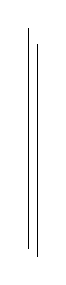
\begin{tikzpicture}\draw (0,0)--(0,2.8);\draw (.12,-.1)--(.12,2.6);\end{tikzpicture}}

\uline{Corollaire} $\mathcal F$ a un plus petit élé\deleted{\unsure{ment|mt}} (savoir, le $\mathrm{Sup}$ de la famille vide d'objets)

\uline{NB} En présence de \deleted{\unsure{C2}} \uline{C 1 b)}, la validité de a) \uline{équivaut} à celle du corollaire.

Le plus petit \unsure{élémt|élément} est appelé \uline{figure vide}, \unsure{notée|noté} $\phi_{\mathcal F}$ ou simplement $\phi$, par abus de langage, et si confusion n'est à craindre

\deleted{\unsure{Réun.|Fam.|Réun} \unsure{des|de} figures comp.

\uline{Définition} \uline{figure} \uline{irréductible $F$ : telle}

que\qquad si\qquad $F=\mathrm{Sup}$}

Figures \uline{compatibles}, ens de figures \deleted{\unsure{compatibles}} compatibles : \deleted{\unsure{un qui|qui}} \inserted{\unsure{dans|de} leur ens.} (\unsure{ou|en} \uline{configuration}) : qui est majoré pour $\leq$. \margin{P} Figure engendrée, ou \uline{réunion} ($F\vee G$, $\bigvee_i f_i$, $\mathrm{Sup}\,F_i$, parfois noté $F\cup G$ \unsure{ou|--} $\deleted{F}\bigcup_iF_i$ cf plus bas).

\uline{Déf} \uline{Figure irréductible} $F$ : telle que $\displaystyle F=\underset{i\in I}{\mathrm{Sup}}\,F_i\ \overset{-}{\Longrightarrow}\ \exists i\in I,\ F_i=F$.

\deleted{\uline{C 2}} Les figures irréductibles sont \unsure{appelées} des \uline{multistrates}. \inserted{L'ens des \unsure{multistr. est|multistrates} noté $ M$} Les figures irréductibles
